\section{Data Model}
\label{sec:model}

A data model consists of a query language, the representation of the
objects on which the language operates, an update language, and a
mechanism for integrity constraints.  In this section we describe the
representation, while Section~\ref{sec:algebra} focuses on the query
language.

We assume linearly ordered, discrete time domain where time instances
have limited precision.  Following the SQL:2011
standard~\cite{DBLP:journals/sigmod/KulkarniM12}, a period (or
interval) $\bp = [s, e)$ represents a discrete contiguous set of time
  instances, starting from and including the start time $s$,
  continuing to but excluding the end time $e$.  A temporal relation
  schema contains a temporal attribute in addition to the nontemporal
  attributes, and we refer to this attribute as $\bp$.

\begin{figure}[t!]
\centering
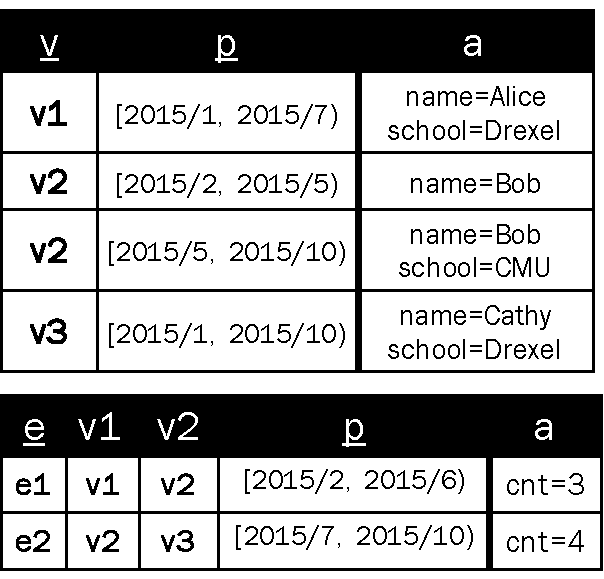
\includegraphics[width=2in]{figs/T1_rel.pdf}
\caption{\tg \insql{T1}.}
\vspace{-0.5cm}
\label{fig:tg_ve}
\end{figure}

We now describe the logical representation of an evolving graph,
called a \tg.  A \tg represents a single graph, and models evolution
of its topology and of vertex and edge attributes.  A \tg is
represented with two temporal
relations~\cite{DBLP:conf/vldb/BohlenSS96}, and uses point
semantics~\cite{DBLP:reference/db/Toman09}, associating a fact
(existence of a vertex or edge, and an assignment of a value to a
vertex or edge attribute) with a time point.  We use periods to
compactly represent their constituent time points.  This is a common
representation technique, which does not add expressive power to the
data model~\cite{DBLP:conf/ictl/Chomicki94}.

A snapshot of a temporal relation $R$, denoted $\tau^s_c(R)$ (``s''
stands for ``snapshot''), is the state of $R$ at time point $c$.

We use the property graph model~\cite{GraphDB} to represent vertex and
edge attributes: each vertex and edge during period $\bp$ is
associated with a (possibly empty) {\em set} of properties, and each
property is represented by a key-value pair.  Property values are not
restricted to be of atomic types, and may, e.g., be sets, maps or
tuples.  Figure~\ref{fig:tg_ve} gives an example of a \tg that shows evolution
of a co-authorship network.

We now give a formal definition of a \tg.

\begin{definition}[TGraph]
A \tg is a pair $\tve=(\tv, \te)$. \tv is a valid-time temporal
relation with schema $\tv(\underline{v}, \underline{\bp}, a)$ that
associates a vertex and its attribute set with the time period during
which it is present and unchanged. \te is a valid-time temporal
relation with schema $\te(\underline{e}, v_1, v_2, \underline{\bp},
a)$, connecting pairs of vertices from \tv.
%
Relations of \tve must meet the following requirements:

\begin{description}[noitemsep]
\item [R1: Unique vertices/ edges] In every snapshot $\tau^s_c (\tv)$
  and $\tau^s_c (\te)$, where $c$ is a time point, a vertex/edge
  exists at most once.  That is, we require set-based semantics with
  duplicate free temporal relations.
\item [R2: Referential integrity] In every snapshot $\tau^s_c (\tve)$,
  foreign key constraints hold from $\tau^s_c (\te)$ to $\tau^s_c
  (\tv)$ on both $v_1$ and $v_2$.
\item [R3: Coalesced] Value-equivalent tuples in all relations of \tve
  with consecutive or overlapping time periods are merged.  
\end{description}
\label{def:tg}
\vspace{-0.5cm}
\end{definition}

Requirements {\bf R1 and R2} guarantee soundness of the \tg data
structure, ensuring that every snapshot of a \tg is a valid graph.
Requirement {\bf R3} avoids semantic ambiguity and ensures correctness
of algebraic operations in point-stamped temporal models such as
ours~\cite{DBLP:reference/db/JensenS09k}.

Graphs may be directed or undirected.  For undirected graphs we choose
a canonical representation of an edge, with $v_1 \leq v_2$ (self-loops
are allowed).  Any number of edges can exist between any two vertices
at any time point, provided they have different ids.  That is, we
support multigraphs.

In the \tg representation of Definition~\ref{def:tg}, vertex and edge
attributes are stored as collections of properties.  That said,
Definition~\ref{def:tg} presents a {\em logical} data structure that
admits different physical representations, including, e.g., a columnar
representation (each property in a separate relation, supporting
different change rates), by a hash-based representation
of~\cite{DBLP:conf/sigmod/SunFSKHX15}, or in some other way.

